174. \begin{figure}[ht!]
\center{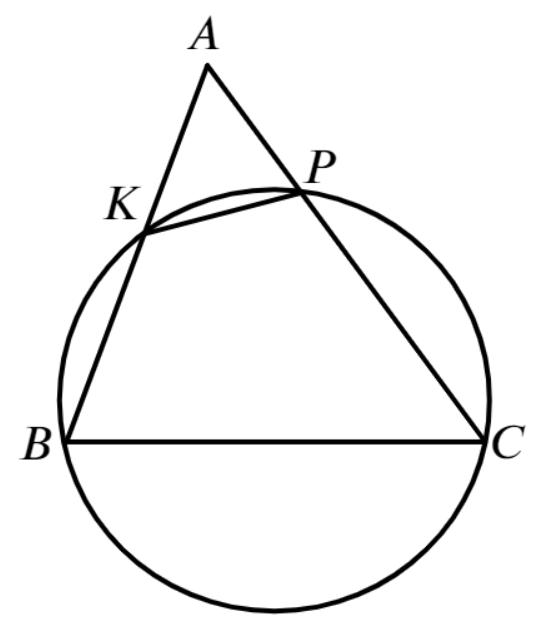
\includegraphics[scale=0.35]{g8-174.png}}
\end{figure}\\
Четырёхугольник $BKPC$ является вписанным, поэтому $\angle B+\angle KPC=180^\circ.$ При этом и $\angle KPA+\angle KPC=180^\circ,$ а значит $\angle B=\angle KPA$ и треугольники $ABC$ и $APK$ подобны по двум углам ($\angle A$ --- общий), откуда $\cfrac{KP}{BC}=\cfrac{AK}{AC},\ KP=\cfrac{BC\cdot AK}{AC}=\cfrac{6}{1,5}=4$см.\\
